\documentclass[main.tex]{subfiles}

\begin{document}


\section{\LaTeX{} Basics \& Best Practices}

\begin{frame}[fragile]{\LaTeX{} Basics}
	\begin{itemize}
		\item Nutzt die Compile-Option \texttt{-output-directory=...}
		      \pause
		      \bigskip
		      \begin{center}
			      \begin{minipage}{0.33\textwidth}
				      \begin{figure}[H]
					      \centering
					      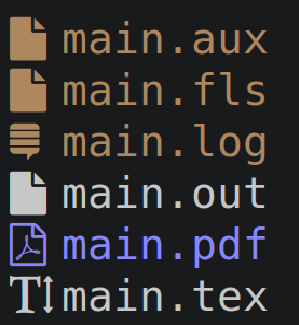
\includegraphics[height=2cm]{images/CompileOutput}
					      \label{fig:CompileOutput}
				      \end{figure}
			      \end{minipage}
			      %
			      \begin{minipage}{0.055\textwidth}
				      →
			      \end{minipage}
			      %
			      \begin{minipage}{0.33\textwidth}
				      \begin{figure}[H]
					      \centering
					      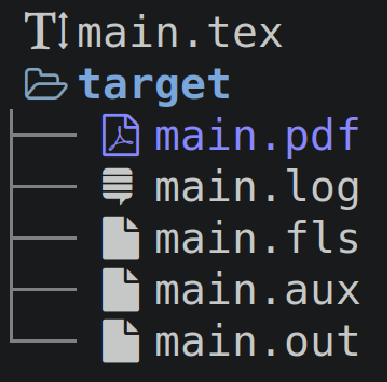
\includegraphics[height=2cm]{images/CompileOutputWithTarget}
					      \label{fig:CompileOutputWithTarget}
				      \end{figure}
			      \end{minipage}
		      \end{center}
		      \pause

		      \bigskip
		\item Nutzt das Paket \texttt{\href{https://tex.stackexchange.com/a/677}{\textbackslash usepackage[T1]\{fontenc\}}}
		      \pfeil{Per default hat \LaTeX{} keinen Support für Umlaute im PDF}
		      \pause
		      \medskip
		\item Bei großen Dokumenten: Dinge modular gestalten
		      \begin{itemize}
			      \item \verb|\include|
			      \item Präambel von Dokument trennen
			      \item Einzelne Abschnitte in verschiedene Dateien auslagern
		      \end{itemize}

	\end{itemize}
\end{frame}



\begin{frame}[fragile]{\LaTeX{} Basics: Versionskontrolle}
	\begin{itemize}
		\item Kennt ihr das?
		      \begin{itemize}
			      \item \verb|präsentation.tex|
			            \pause
			      \item \verb|präsentation_v2.tex|
			            \pause
			      \item \verb|präsentation_final.tex|
			            \pause
			      \item \verb|präsentation_final_final.tex|
			            \pause
			      \item \verb|präsentation_final_final_korrigiert.tex|
		      \end{itemize}
		      \medskip
		      \pause
		\item Es ist schwer zu wissen,
		      \begin{itemize}
			      \item welche Datei die aktuellste ist
			      \item was sich zwischen den Versionen verändert hat
			      \item wer welche Änderungen vorgenommen hat
		      \end{itemize}
		      \pause
		      \medskip
		\item[$\to$] Versionskontrolle verwenden\pause: git\pause, overleaf\pause, subversion
	\end{itemize}

\end{frame}

\begin{frame}[fragile]{\LaTeX{} Basics: Referenzen}
	\begin{itemize}
		\item[1.] Paket \verb|\usepackage{hyperref}| verwenden
			\pause
		\item[2.] Label setzen
			\pause
		\item[3.] Label referenzieren
			\medskip
			\pause
		\item Falls deutsche Labels verwendet werden sollen: \verb|\usepackage[ngerman]{babel}|
		      \pause
		      \medskip
		\item Vor Referenzen immer ein \emph{unbreakable space} \verb|(~)| verwenden
		      \begin{itemize}
			      \item[$\to$] \verb|In~\cref{fig:cat} ist eine Katze zu sehen|
		      \end{itemize}
	\end{itemize}
\end{frame}

\begin{frame}{\LaTeX{} Basics: Referenzen -- Beispiel}
	\begin{minipage}[t][][b]{0.49\textwidth}
		\begin{table}[h]
			\centering
			\begin{tabular}{|c|c|c|}
				\hline
				\textbf{A} & \textbf{B} & \textbf{C} \\
				\hline
				1          & 2          & 3          \\
				\hline
				4          & 5          & 6          \\
				\hline
				7          & 8          & 9          \\
				\hline
			\end{tabular}
			\vspace{42pt}
			\caption{Dummy-Tabelle}
			\label{tab:dummy}
		\end{table}
	\end{minipage}
	%
	\begin{minipage}[t][][b]{0.49\textwidth}
		\begin{figure}
			\centering
			
\includegraphics[width=0.5\textwidth]{images/DummyCatPicture}
			\caption{Dummy-Bild}
			\label{fig:dummy}
		\end{figure}
	\end{minipage}

	\begin{align}
		1+1 & = 2 \label{eq:dummy}
	\end{align}
\end{frame}

\def\makeReferenceCompareTable#1#2#3{
	\begin{table}[H]
		\centering
		\begin{tabularx}{\textwidth}{{>{\ttfamily}L{130pt}X}}
			\toprule
			\textbf{Command}                     & \textbf{Output}            \\
			\midrule
			\textbackslash ref\{…\}              & \ref{#1}                   \\
			\textbackslash nameref\{…\}          & \hyperref[#1]{#3}          \\
			\textbackslash autoref\{…\}          & \hyperref[#1]{#2 \ref{#1}} \\
			\textbackslash hyperref[<name>]\{…\} & \texttt{<name>}            \\
			\textbackslash vref\{…\}             & \vref{#1}                  \\
			\textbackslash cref\{…\}             & \cref{#1}                  \\
			\textbackslash Cref\{…\}             & \Cref{#1}                  \\
			\bottomrule
		\end{tabularx}
		\label{tab:DifferentWaysOfRefencing (#1)}
	\end{table}
}

\begin{frame}[fragile]{\LaTeX{} Basics: Vergleich von Referenz-Commands (Tabellen)}
	\makeReferenceCompareTable{tab:dummy}{Tabelle}{Dummy-Tabelle}
\end{frame}

\begin{frame}[fragile]{\LaTeX{} Basics: Vergleich von Referenz-Commands (Figuren)}
	\makeReferenceCompareTable{fig:dummy}{Abbildung}{Dummy-Bild}
\end{frame}

\begin{frame}[fragile]{\LaTeX{} Basics: Vergleich von Referenz-Commands (Gleichungen)}
	\makeReferenceCompareTable{eq:dummy}{Gleichung}{\texttt{<section-name>}}
\end{frame}

\begin{frame}[fragile]{\LaTeX{} Basics: Referenzen -- Welches Makro?}
	\begin{itemize}
		\pause
		\item Eigentlich immer cleveref\medskip
		      \pause
		\item \ldots{} Aber welches Makro? \verb|\cref| oder \verb|\Cref|?
		      \pause
		      \begin{itemize}
			      \item[$\to$] Keinen Unterschied im \textit{Deutschen}
			      \item Im Englischen macht \verb|\cref| einen Kleinbuchstaben
		      \end{itemize}
		      \pause
		      \medskip
		\item \verb|\autoref| geht auch, oft den gleicher Output wie cleveref
	\end{itemize}
\end{frame}



\begin{frame}[fragile]{\LaTeX{} Basics: Wann sollte ich welchen Dash verwenden?}
	\begin{table}
		\centering
		\begin{tabular}{|c|c|c|c|}
			\hline
			Dash & In \LaTeX  & Deutscher Name       & Englischer Name \\\hline
			-    & \verb|-|   & Viertelgeviertstrich & hyphen          \\\hline
			--   & \verb|--|  & Halbgeviertstrich    & en-dash         \\\hline
			---  & \verb|---| & Geviertstrich        & em-dash         \\\hline
		\end{tabular}
		\label{tab:WannWelchenDash}
	\end{table}
	\pause
	\vspace{-7pt}

	\begin{onlyenv}<-5>
		\begin{itemize}
			\uncover<2->{\item \href{http://www.schriftdeutsch.de/ortr-bin.htm}{\textbf{Deutsch}}}
			      \begin{itemize}
				      \begin{uncoverenv}<3->
					      \item \verb|-| zwischen Wörtern:\\\enquote{Mein Lieblingssport ist Schach-Boxen.}
				      \end{uncoverenv}
				      \medskip
				      \begin{uncoverenv}<4->
					      \item \verb|--| für Einschübe und Zahlenbereiche / Ranges:\\\enquote{Meine Oma – die übrigens auch ein hervorragendes Strudelrezept hat – kommt morgen zu Besuch.}
					      \\\enquote{Die Teilnehmerzahl liegt zwischen 50--100 Personen.}
				      \end{uncoverenv}

				      \medskip
				      \begin{uncoverenv}<5->
					      \item \verb|---| wird oft als störend empfunden, kaum genutzt
				      \end{uncoverenv}
			      \end{itemize}
		\end{itemize}
	\end{onlyenv}

	\begin{onlyenv}<6->
		\begin{itemize}
			\uncover<6->{\item \href{https://tex.stackexchange.com/a/3821}{\textbf{Englisch}}}
			      \begin{itemize}
				      \begin{uncoverenv}<7->
					      \item \verb|-| zwischen Wörtern:\\`The rock-paper-scissors-lizard-Spock game is really fun.'
				      \end{uncoverenv}
				      \medskip
				      \begin{uncoverenv}<8->
					      \item \verb|--| für Zahlenbereiche / Ranges:\\`I can count from 1--10 in five different languages.'
				      \end{uncoverenv}

				      \medskip
				      \begin{uncoverenv}<9->
					      \item \verb|---| für Einschübe:\\`I absolutely adore penguins---those waddling, tuxedo-wearing birds---they always make me smile.'
					      \pfeil{Traditionell: heutzutage manchmal auch en-dash mit spaces}
				      \end{uncoverenv}
			      \end{itemize}
		\end{itemize}
	\end{onlyenv}
\end{frame}


\begin{frame}{\LaTeX{} Basics: Code-Listings -- Flowchart}
	\vspace{-25pt}
	\begin{tikzpicture}
		[
			circ/.style={circle, draw, minimum height=1cm, minimum width=2cm},
			ellip/.style={ellipse, draw, minimum height=1cm, minimum width=2cm},
			arrow/.style={->,>=stealth},
			every initial by arrow/.style=arrow,
			every accepting by arrow/.style=arrow,
		]
		\node[circ] (code listing) at (0, 0) {\makecell{Code-\\Listing}};
		\node[above=1/2 of code listing] (code listing init) {};
		\draw[arrow] (code listing init) -- (code listing);
		\pause

		\node[ellip, below left=of code listing] (kein syntax highlighting) {\makecell{Kein Syntax-\\Highlighting}};
		\draw[arrow] (code listing) -- (kein syntax highlighting);
		\pause

		\node[ellip, below right=of code listing] (syntax highlighting) {\makecell{Syntax-\\Highlighting}};
		\draw[arrow] (code listing) -- (syntax highlighting);
		\pause

		\node[circ, below left=2/3 of kein syntax highlighting, yshift=-0.5cm] (kein escaping) {\makecell{Kein\\Escaping}};
		\node[circ, below right=2/3 of kein syntax highlighting, yshift=-0.5cm] (escaping) {\makecell{Escaping}};

		\draw[arrow] (kein syntax highlighting) -- (kein escaping);
		\draw[arrow] (kein syntax highlighting) -- (escaping);

	\end{tikzpicture}
\end{frame}

\begin{frame}[fragile]{\LaTeX{} Basics: Code-Listings (ohne Syntax Highlighting)}
	\begin{itemize}
		\item \LaTeX-Befehl \verb|\texttt|
	\end{itemize}
	\pause
	\vspace{-10pt}
	\begin{center}
		\begin{verbatim}
            \texttt{print("Hello, world!")}
        \end{verbatim}
		\vspace{-17pt}
		↓

		\texttt{print("Hello, world!")}
	\end{center}
	\pause
	\vspace{-7pt}
	\begin{itemize}
		\item Aber:
	\end{itemize}
	\pause
	\vspace{-10pt}
	\begin{center}
		\begin{verbatim}
            \texttt{printf("Hello, %s!", name)}
        \end{verbatim}
		\vspace{-17pt}
		↓

		\textcolor{red}{Fatal error occurred, no output PDF file produced!}
	\end{center}
\end{frame}



\begin{frame}[fragile]{\LaTeX{} Basics: Code-Listings (ohne Syntax Highlighting)}
	\begin{itemize}
		\item Automatisches Escaping
		      \pause
		\item Verbatim Paket: \verb|\usepackage{verbatim}|
	\end{itemize}
	\pause
	\vspace{-10pt}
	\begin{center}
		\begin{verbatim}
          \verb|printf("Hello, %s!", name)|
        \end{verbatim}
		\vspace{-17pt}
		↓

		\verb|printf("Hello, %s!", name)|
	\end{center}
	\pause
	\vspace{-7pt}
	\begin{itemize}
		\item Auch als Umgebung:
	\end{itemize}
	\pause
	\vspace{-10pt}
	\begin{center}
		% TODO: Fix indentation
		\begin{metaverbatim}
			\begin{verbatim}
              printf("Hello, %s!", name)
            \end{verbatim}
		\end{metaverbatim}
		\vspace{-30pt}
		↓

		\verb|printf("Hello, %s!", name)|
	\end{center}
\end{frame}

\begin{frame}[fragile]{\LaTeX{} Basics: Code-Listings (mit Syntax Highlighting)}
	\begin{itemize}
		\item Listings
		      \uncover<2->{
			      \begin{itemize}
				      \item Rudimentäres Syntax Highlighting (Keyword-Highlighting)
				      \item Relativ Langsam, ziemlich alt, geschrieben in \TeX
				      \item Muss Customized werden
				      \item Probleme mit Unicode
			      \end{itemize}
		      }
		      \medskip
		\item \href{https://tex.stackexchange.com/a/389221}{minted}
		      \uncover<3->{
			      \begin{itemize}
				      \item Sehr feature-reich (Kontext-Highlighting)
				      \item Powered by Pygments
				            \medskip
				      \item Unterstützt mehr Programmiersprachen
				      \item Benötigt System Setup
				            \pfeil{Python, Pygments und Compiler-Option \verb|-shell-escape|}
			      \end{itemize}
		      }
	\end{itemize}
\end{frame}

\begin{frame}[fragile]{\LaTeX{} Basics: Code-Listings (listings)}
	\begin{lstlisting}[language=Python]
def greet(name: str):
    message = f"Hello, {name}!"
    return message

def fibonacci(n: int):
    if n <= 1:
      return n
    else:
      return fibonacci(n-1) + fibonacci(n-2)

def is_palindrome(s: str):
    s = s.lower().replace(" ", "")
    return s == s[::-1]
    \end{lstlisting}
\end{frame}

\begin{frame}[fragile]{\LaTeX{} Basics: Code-Listings (minted)}
	\begin{minted}[style=autumn]{python}
def greet(name: str):
    message = f"Hello, {name}!"
    return message

def fibonacci(n: int):
    if n <= 1:
        return n
    else:
        return fibonacci(n - 1) + fibonacci(n - 2)

def is_palindrome(s: str):
    s = s.lower().replace(" ", "")
    return s == s[::-1]
    \end{minted}
\end{frame}

\begin{frame}[fragile]{\LaTeX{} Basics: Code-Listings (listings)}
	\begin{lstlisting}
fn greet(name: &str) -> String {
    format!("Hello, {name}!")
}

fn fibonacci(n: u32) -> u32 {
    match n {
        0 | 1 => n,
        _ => fibonacci(n-1) + fibonacci(n-2)
    }
}

fn is_palindrome(s: &str) -> bool {
  let s = s.to_lowercase().replace(" ", "");
  s == s.chars().rev().collect::<String>()
}
    \end{lstlisting}
\end{frame}

\begin{frame}[fragile]{\LaTeX{} Basics: Code-Listings (minted)}
	\begin{minted}[style=autumn]{Rust}
fn greet(name: &str) -> String {
    format!("Hello, {name}!")
}

fn fibonacci(n: u32) -> u32 {
    match n {
        0 |\textbar| 1 => n,
        _ => fibonacci(n - 1) + fibonacci(n - 2)
    }
}

fn is_palindrome(s: &str) -> bool {
    let s = s.to_lowercase().replace(" ", "");
    s == s.chars().rev().collect::<String>()
}
    \end{minted}
\end{frame}



\begin{frame}[fragile]{\LaTeX{} Mathe-Basics}
	\begin{itemize}
		\item Mit dem \texttt{\$} wird der \textit{inline} Mathe-Modus eingeleitet
		      \pause
		      \begin{center}
			      \verb|$a = -b$| wird zu $a=-b$
		      \end{center}
		      \pause
		\item Der \textit{display} Mathe Modus wird mit \verb|\[ ... \]| eingeleitet
		      %
		      \vspace{-7pt}
		      \begin{center}
			      \begin{minipage}[t][][b]{0.35\textwidth}
				      \begin{verbatim}
\[ a = -b \]
                \end{verbatim}
			      \end{minipage}
			      %
			      \begin{minipage}[t][][b]{0.35\textwidth}
				      \vspace{-9pt}\[a = -b\]
			      \end{minipage}
		      \end{center}
		      \vspace{-7pt}
		      \pause
		\item Statt \verb|$$ ... $$| lieber \verb|\[ ... \]| \href{https://tex.stackexchange.com/a/69854}{verwenden}
		      \pause
		      \medskip
		\item Durch \verb|\usepackage{amsmath}| auch durch \texttt{align} möglich
		      \pause
		      \vspace{-7pt}
		      \begin{center}
			      \begin{minipage}[t][][b]{0.35\textwidth}
				      \begin{verbatim}
\begin{align}
         a &= b \\
  \sqrt{2} &= c
\end{align}
                \end{verbatim}
			      \end{minipage}
			      %
			      \begin{minipage}[t][][b]{0.35\textwidth}
				      \vspace{-6pt}
				      \begin{align}
					      a        & = b \\
					      \sqrt{2} & = c
				      \end{align}
			      \end{minipage}
		      \end{center}
		      \vspace{-7pt}
	\end{itemize}
\end{frame}


\begin{frame}[fragile]{\LaTeX{} Mathe-Basics: Symbole}
	\def\mathVis#1{$\csname #1\endcsname\,(\texttt{\textbackslash #1})$}
	\def\mathVisBB#1{$\mathbb{#1}\,(\texttt{\textbackslash mathbb\{#1\}})$}
	\def\mathVisDS#1{$\mathds{#1}\,(\texttt{\textbackslash mathds\{#1\}})$}

	\begin{itemize}
		\item Verschiedene Kategorien
		      \begin{itemize}
			      \item Gleichzeichen: $=$, \mathVis{neq}, \mathVis{approx}
			      \item Griechische Buchstaben: \mathVis{alpha}, \mathVis{beta}
			      \item Mathematische Operatoren: \mathVis{sum}, \mathVis{int}
			      \item Zahlenmengen: \mathVisBB{N} oder \mathVisDS{N}
			      \item Pfeile: \mathVis{to}, \mathVis{Rightarrow}, \mathVis{mapsto}
		      \end{itemize}
		      \pause
		\item Falls dein Zeichen hier nicht dabei war: \href{https://detexify.kirelabs.org/classify.html}{Detexify}
		      \pause
		      \medskip
		\item Welches der Symbole findet ihr besser? $\mathbb{N}$ oder $\mathds{N}$
		      \pause
		      \begin{itemize}
			      \item $\mathds{N}$ ist eher handschriftlich
			            \pause
			      \item Falls euch etwas vorgeschrieben wird, nehmt das
			            \pause
			      \item Ansonsten: Nehmt das was ihr möchtet.\\\quad \textcolor{red}{Aber haltet euch dran!}
		      \end{itemize}
	\end{itemize}
\end{frame}


\begin{frame}[fragile]{\LaTeX{} Mathe-Basics: Was ist hier falsch?}

	\only<3, 6, 9>{
		\begin{itemize}
			\only<3, 6, 9>{
			\item Das Spacing zwischen dem Strich ist zu wenig
			\item Wie geht es besser? \texttt{\textbackslash mid}
			      }
			      \bigskip
			      \only<6, 9>{
			\item Das = und der Doppelpunkt sind nicht aligned
			\item Wie geht es besser? \texttt{\textbackslash coloneq}
			      }
			      \bigskip
			      \only<9>{
			\item Das \textit{sin} sollte nicht kursiv geschrieben sein
			\item Wie geht es besser? \texttt{\textbackslash sin}
			      }
		\end{itemize}
	}

	\only<1-3>{
		\begin{center}
			\only<1-3>{
				\begin{minipage}[t][][b]{0.40\textwidth}
					\fontsize{20}{1}\selectfont   $\{x\in \mathbb{N} \textbar x > 5 \}$
				\end{minipage}
				\only<4-5>{\vspace{50pt}}
			}
			\only<2-3>{
				\begin{minipage}[t][][b]{0.45\textwidth}
					\fontsize{20}{1}\selectfont  $\{x\in \mathbb{N} \mid x > 5 \}$
				\end{minipage}
			}
		\end{center}
	}

	\only<4-6>{
		\begin{center}
			\only<4-6>{
				\begin{minipage}[t][][b]{0.25\textwidth}
					\fontsize{20}{1}\selectfont   $a := 5$
				\end{minipage}
				\only<1-2>{\vspace{50pt}}
			}
			\only<5-6>{
				\begin{minipage}[t][][b]{0.25\textwidth}
					\fontsize{20}{1}\selectfont$a \coloneq 5$
				\end{minipage}
			}
		\end{center}
	}

	\only<7-9>{
		\begin{center}
			\only<7-9>{
				\begin{minipage}[t][][b]{0.35\textwidth}
					\fontsize{20}{1}\selectfont   $sin(x)$
				\end{minipage}
				\only<7-8>{\vspace{50pt}}
			}
			\only<8-9>{
				\begin{minipage}[t][][b]{0.35\textwidth}
					\fontsize{20}{1}\selectfont  $\sin(x)$
				\end{minipage}
			}
		\end{center}
	}

\end{frame}


\begin{frame}{\LaTeX{} Mathe-Basics: Wann sollte was kursiv sein?}
	\begin{itemize}
		\item Ausgehend von \href{https://physics.nist.gov/cuu/pdf/typefaces.pdf}{NIST} \ldots
		      \pause
		      \medskip
		\item Mathematische Funktionen sollten \textit{nicht} kursiv sein
		      \pfeil{$tan(x)$ vs.\ $\tan(x)$, $exp(x)$ vs.\ $\exp(x)$}
		      \pause

		\item Variablen und Funktionen mit 1 Buchstaben sollten kursiv sein
		      \pfeil{$x, y, z, t, r, \lambda, f(x)$}
		      \pause

		\item Einheiten sollten \textit{nicht} kursiv sein
		      \pfeil{$t=3 \textrm{s}$, $r=11 \textrm{cm}$, $\lambda = 420 \textrm{nm}$}
		      \pause

		\item Mathematische Konstanten werden nicht kursiv geschrieben
		      \pfeil{$\e^{\i\cdot \pI} = -1$}
		      \pause

		\item Der Differentialoperator sollte nicht kursiv sein
		      \pfeil{$\int\limits_{a}^{b} x^2 dx$ vs.\ $\int\limits_{a}^{b} x^2 \textrm{d}x$,\quad $f'(x) = \frac{df(x)}{dx}$ vs.\ $f'(x) = \frac{\textrm{d}f(x)}{\textrm{d}x}$}
	\end{itemize}
\end{frame}

\end{document}
